\section{Results}
\label{sec:results}

\subsection{The spectrum}
\label{sec:spectrum-desc}

\Cref{fig:spectrum} shows the familiar picture. In the full sample the
market mode carries $\lambda_0=\FullLamZero$, or \FullLamZeroShare\% of
total variance, and its eigenvector is almost exactly the equal-weight
portfolio (overlap \FullOverlap). Once the bulk is rescaled for the
variance absorbed by the market mode \citep{laloux1999}, the remaining
eigenvalues sit close to the Marchenko--Pastur density, with
\FullNSigRescaled{} modes above the edge. In the rolling 252-day windows
($q=\RollQ$) the edge is $\lambda_+=\RollMPUpper$. Between 3 and 11
modes clear it, a handful of sector-like factors behind the market
mode, and everything else is statistically indistinguishable from
noise. (The walk-forward uses the unrescaled, conservative edge with
$\sigma^2=1$. The rescaled edge admits about 13 modes per window, all
inside Pool~A, and changes none of the conclusions below.)

\begin{figure}[t]
\centering
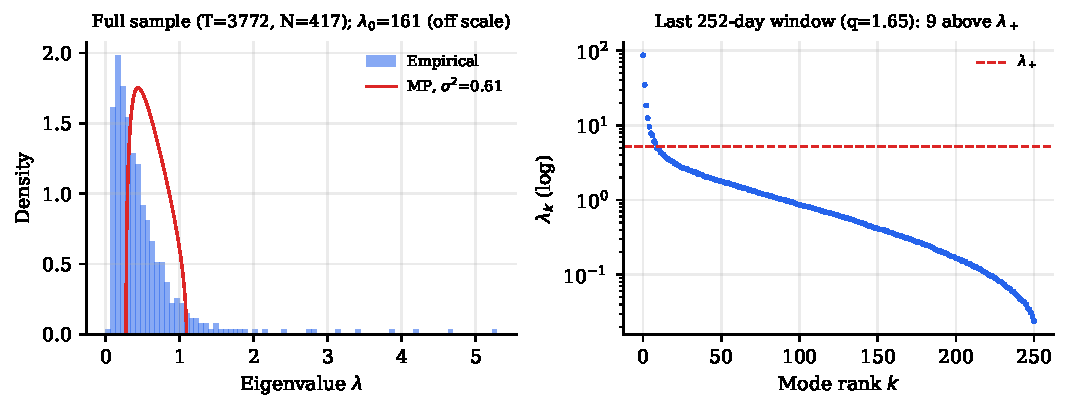
\includegraphics[width=\textwidth]{spectrum}
\caption{Left: full-sample eigenvalue density against the Marchenko--Pastur
law, rescaled for the variance absorbed by the market mode. Right:
eigenvalues of the last 252-day window on a log scale, with the edge
$\lambda_+$ used in the walk-forward. Beyond rank $T-1=251$ the
eigenvalues are exactly zero.}
\label{fig:spectrum}
\end{figure}

\subsection{Where is the mean reversion?}
\label{sec:spectrum}

Our first test uses no machine learning. In every episode we trade the
standalone reversion signal \eqref{eq:signal} on \emph{every}
non-degenerate mode, normalize each mode's PnL by $\sqrt{\lambda_k}$,
and average within buckets defined relative to that episode's own MP
edge $n_s$. \Cref{tab:spectrum} and \cref{fig:spectrum-reversion}
report out-of-sample (2013--2024), pre-cost results.

\begin{table}[t]
\centering\small
\caption{Out-of-sample standalone reversion by position in the spectrum,
2013--2024, before costs. Buckets are defined relative to each episode's
MP edge $n_s$. Sharpe ratios are annualized for an equal-risk portfolio
of the modes in the bucket; $t_{NW}$ uses Newey--West standard errors
with 10 lags. The last two columns give the mean out-of-sample lag-1
autocorrelation of daily mode returns within an episode and its $t$-statistic
across episodes.}
\label{tab:spectrum}
\begin{tabular}{lrrrrrr}
\toprule
 & \multicolumn{2}{c}{Level reversion} & \multicolumn{2}{c}{Return reversal} & \multicolumn{2}{c}{OOS lag-1 AC} \\
\cmidrule(lr){2-3}\cmidrule(lr){4-5}\cmidrule(lr){6-7}
Modes & Sharpe & $t_{NW}$ & Sharpe & $t_{NW}$ & $\bar\rho_1$ & $t$ \\
\midrule
Market ($k=0$) & -0.09 & -0.33 & 0.18 & 0.56 & -0.066 & -4.06 \\
Signal, above MP ($1..n_s-1$) & 0.07 & 0.26 & -0.57 & -1.96 & -0.047 & -6.33 \\
Edge bulk ($n_s..n_s+24$) & -0.00 & -0.02 & -0.25 & -0.71 & -0.054 & -12.05 \\
Upper bulk ($n_s+25..99$) & 0.54 & 1.86 & 0.63 & 2.89 & -0.057 & -21.71 \\
Middle bulk ($100..174$) & 0.87 & 2.74 & 1.10 & 4.07 & -0.057 & -21.66 \\
Lower bulk ($175..249$) & 0.70 & 2.39 & 0.95 & 3.14 & -0.056 & -22.15 \\
\bottomrule
\end{tabular}
\end{table}

\begin{figure}[t]
\centering
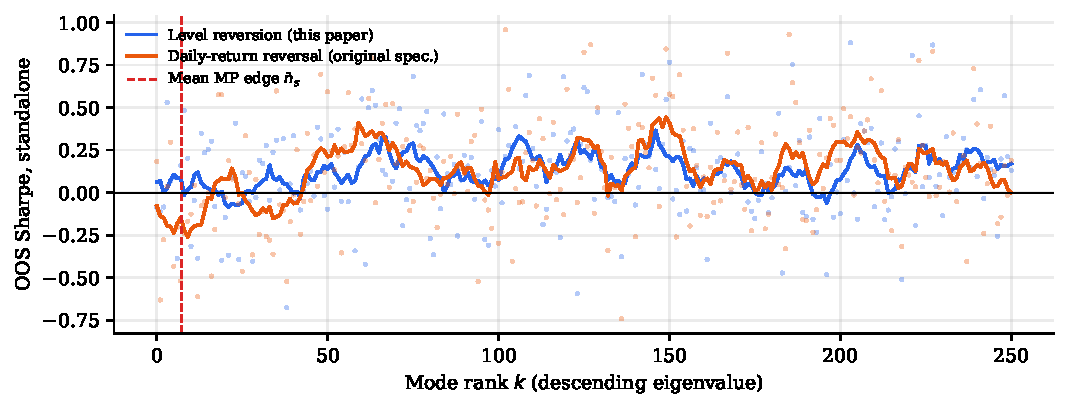
\includegraphics[width=\textwidth]{spectrum_reversion}
\caption{Out-of-sample Sharpe ratio of the standalone reversion signal for
each mode rank (dots) and a 9-mode moving average (lines), 2013--2024,
before costs. The dashed line marks the average MP edge.}
\label{fig:spectrum-reversion}
\end{figure}

Three results stand out.

\emph{First, the modes that random matrix theory certifies as signal do
not mean-revert in a tradable way.} The level-reversion Sharpe ratio of
the above-MP modes is \SRSignalLevel{} ($t=\TSignalLevel$). For the
first 25 modes below the edge it is \SREdgeLevel{}. The original
repository's daily-return reversal signal does worse on the signal
modes (\SRSignalRet, $t=\TSignalRet$): these portfolios are sector-like
factors that trend over days rather than revert.

\emph{Second, reversion lives in the bulk.} The Sharpe ratio rises to
\SRUpperLevel{} for modes $n_s+25$ to 99, \SRMiddleLevel{} for modes
100--174 ($t=\TMiddleLevel$) and \SRLowerLevel{} for the lowest modes
($t=\TLowerLevel$). The same pattern, slightly stronger, holds for the
return-reversal signal (\SRMiddleRet, $t=\TMiddleRet$). Purely
statistically, every bucket has negative out-of-sample lag-1
autocorrelation. For the market and signal modes it is about $-0.05$
($t\approx\ACtSignal$), and in the bulk it is about \ACMiddle{} with
$t$-statistics above 20 in absolute value. Mode returns at the bottom
of the spectrum reverse day to day, as the overdamped picture of
\cref{sec:theory} suggests. The reversal is economically small: a lag-1
autocorrelation of $-0.06$ explains well under 1\% of next-day variance.

\emph{Third, the simple OU prediction for half-lives fails.}
Equation~\eqref{eq:prediction} predicts that the in-window half-life
rises one-for-one with $\lambda_k$ on a log scale. The fitted slope
across all modes and episodes is \OUSlope{}, and the Spearman correlation
is \OUSpearman{} (\cref{fig:ou} in the appendix). The 252-day AR(1)
half-life of the level is a poor statistic for day-scale reversal, and
the lowest-variance sample eigenvectors are partly artefacts of
estimation noise, whose in-sample variance is biased downward
\citep{bunbouchaud2017}. The qualitative ordering of
\eqref{eq:equipartition}, with stiff directions reverting faster, shows
up in out-of-sample \emph{profitability}, not in in-sample half-lives.

These findings reframe the original thesis. The intuition that the
``smallest signal modes'' are the natural building blocks of a reversion
portfolio is right about direction (small eigenvalues) but wrong about
where to stop. The MP filter discards exactly the part of the spectrum
where reversion is concentrated.

\subsection{Can mode quality be predicted?}
\label{sec:ml-results}

The base rate is high, with \BaseRateA\% of Pool~A mode-months
profitable out of sample. This reflects the negative skew of reversion
payoffs: many small gains and occasional large losses. \Cref{tab:auc}
reports out-of-sample AUCs.

\begin{table}[t]
\centering\small
\caption{Out-of-sample AUC for predicting $y=\mathbf 1\{\pi_k>0\}$,
2013--2024 (\OOSRowsA{} mode-months in Pool~A, \OOSRowsB{} in Pool~B).
Brackets: 95\% intervals from a bootstrap over episodes. Heuristics
rank modes by a single in-window statistic.}
\label{tab:auc}
\begin{tabular}{llcc}
\toprule
Pool & Model & Mode features & Mode + regime features \\
\midrule
Modes 1--30 & Logistic (L2) & 0.523 [0.506, 0.540] & 0.521 [0.501, 0.537] \\
 & Gradient boosting & 0.518 [0.502, 0.535] & 0.518 [0.499, 0.538] \\
 & Random forest & 0.524 [0.508, 0.543] & 0.528 [0.509, 0.545] \\
 & Heuristic: $-\log$ half-life & \multicolumn{2}{c}{0.512} \\
 & Heuristic: $-\log\lambda$ & \multicolumn{2}{c}{0.504} \\
\midrule
Full spectrum & Logistic (L2) & 0.508 [0.500, 0.515] & 0.514 [0.505, 0.522] \\
 & Gradient boosting & 0.506 [0.501, 0.512] & 0.504 [0.497, 0.512] \\
 & Random forest & 0.507 [0.500, 0.513] & 0.512 [0.505, 0.520] \\
 & Heuristic: $-\log$ half-life & \multicolumn{2}{c}{0.512} \\
 & Heuristic: $-\log\lambda$ & \multicolumn{2}{c}{0.493} \\
\bottomrule
\end{tabular}
\end{table}

\begin{table}[t]
\centering\small
\caption{Feature-group importance for the primary (logistic, all-feature)
model. ``Solo AUC'' trains on that group alone; ``$\Delta$AUC (drop)''
is the change in out-of-sample AUC when the group is removed.}
\label{tab:ablation}
\begin{tabular}{lrrrr}
\toprule
 & \multicolumn{2}{c}{Modes 1--30} & \multicolumn{2}{c}{Full spectrum} \\
\cmidrule(lr){2-3}\cmidrule(lr){4-5}
Feature group & Solo AUC & $\Delta$AUC (drop) & Solo AUC & $\Delta$AUC (drop) \\
\midrule
Eigenvalue separation & 0.504 & +0.003 & 0.507 & -0.001 \\
Half-life & 0.510 & +0.002 & 0.508 & -0.001 \\
Autocorrelation & 0.522 & -0.004 & 0.501 & +0.001 \\
Eigenvector stability & 0.506 & -0.000 & 0.498 & +0.000 \\
Volatility & 0.512 & -0.002 & 0.491 & +0.000 \\
Concentration & 0.523 & -0.005 & 0.490 & -0.001 \\
Trailing reversion & 0.511 & +0.001 & 0.497 & +0.000 \\
Regime & 0.506 & +0.002 & 0.512 & -0.006 \\
\bottomrule
\end{tabular}
\end{table}

Predictability is real but small. In Pool~A every model clears 0.5. The
logistic model with mode features reaches \AUCLogitModeA{}
[\AUCLoLogitModeA, \AUCHiLogitModeA], and the random forest with all
features reaches \AUCRfAllA{} [\AUCLoRfAllA, \AUCHiRfAllA]. Gradient
boosting is no better than the linear model, as expected when the
signal-to-noise ratio is this low. In Pool~B, where most rows are bulk
modes that all revert to a similar degree, the AUCs fall to 0.504--0.514.
The single-statistic heuristics score below the multivariate models:
ranking by short half-life gives \AUCHeurHalfLifeA{} in Pool~A, and
ranking by small eigenvalue gives \AUCHeurLambdaA, indistinguishable
from chance.

The ablation in \cref{tab:ablation} shows no single dominant group.
The most informative groups on their own are portfolio concentration
(broad modes revert more reliably than near-pairs) and autocorrelation;
removing any one group changes the AUC by less than 0.006. Adding the
regime features barely changes the AUC, but it does change the
\emph{level} of predicted probabilities. In Pool~A the base rate is
\BaseRateAStress\% in the stress state against \BaseRateACalm\% in the
calm state, and the mean normalized forward PnL is negative in calm
months. Timing, rather than cross-sectional selection, is where the
regime information pays off (\cref{sec:strategy}).

\begin{figure}[t]
\centering
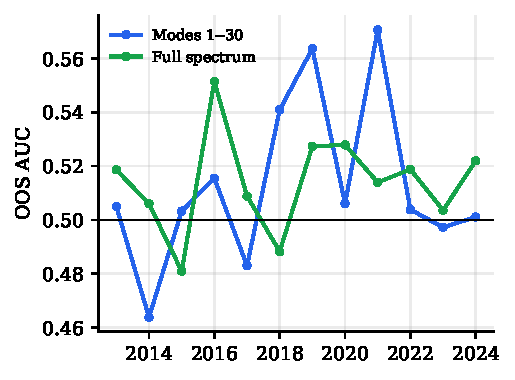
\includegraphics[width=0.5\textwidth]{auc_by_year}
\caption{Out-of-sample AUC by calendar year for the primary model.}
\label{fig:auc-year}
\end{figure}

\begin{figure}[t]
\centering
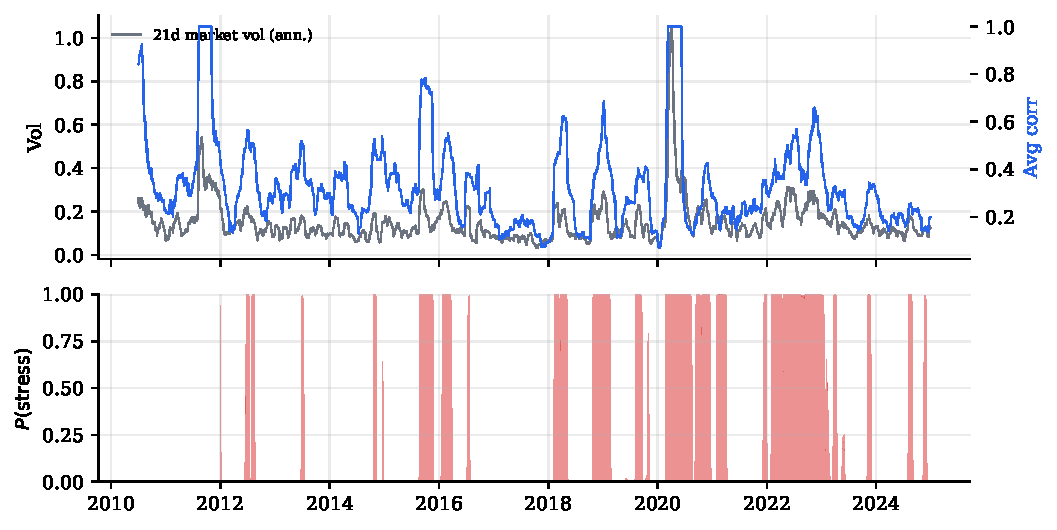
\includegraphics[width=\textwidth]{regimes}
\caption{Regime features (top) and the walk-forward filtered stress
probability (bottom).}
\label{fig:regimes}
\end{figure}

\subsection{Regimes}

The two HMM states are cleanly separated
(\cref{fig:regimes}). In the most recent fit, the calm state
has \CalmVol\% annualized market volatility and an average pairwise
correlation of \CalmCorr, against \StressVol\% and \StressCorr{} in the
stress state. Both states are persistent (daily stay probabilities
\PStayCalm{} and \PStayStress). The filtered stress probability exceeds
one half on \FracStress\% of days: \StressTwentyTwenty\% of 2020,
\StressTwentyTwentyTwo\% of 2022 and \StressTwentySeventeen\% of 2017.

\subsection{Walk-forward strategies}
\label{sec:strategy}

\paragraph{Construction.} In each episode the selected modes are traded
with signal \eqref{eq:signal}, each scaled by $1/\sqrt{\lambda_k}$ for equal
ex-ante risk. Mode positions are mapped to asset weights
$x_i=\sum_k w_k\,s_k\,v_{ik}/(\sqrt{\lambda_k}\sigma_i)$ and rescaled
daily to unit gross exposure. ML strategies select the top third of
each episode's pool by predicted probability. Costs are 2~bp per unit
of one-way turnover. All strategies are evaluated on the same period
(7 January 2013 -- 30 December 2024).

\paragraph{Regime overlay.} The episode-level exposure is
$e_j=(1-p_j)g_{\text{calm}}+p_j g_{\text{stress}}$, where $p_j$ is the
filtered stress probability before the episode and
$g_s=\operatorname{clip}(\widehat{SR}_s/\max_{s'}\widehat{SR}_{s'},0,1)$.
Here $\widehat{SR}_s$ is the strategy's own past gross Sharpe ratio on
days classified to regime $s$, using only completed episodes. The best
regime so far is traded at full size and a regime with a negative past
Sharpe is not traded. \emph{Disclosure:} our pre-specified overlay could
only de-risk in the stress state. It was never active, because the
strategy's past stress-state Sharpe always exceeded its calm-state
Sharpe. The symmetric rule above replaced it after we saw this. The
rule is still strictly walk-forward, but its form was informed by the
data, and its results should be discounted accordingly.

\begin{table}[t]
\centering\small
\caption{Walk-forward strategy performance, 7 January 2013 -- 30 December 2024. Net of
2~bp per unit turnover unless labelled gross. Turnover is average daily
one-way turnover as a fraction of gross exposure. Break-even is the
cost in bp per unit turnover at which the net return is zero.}
\label{tab:strategies}
\resizebox{\textwidth}{!}{\begin{tabular}{llrrrrrrr}
\toprule
Strategy & Pool & Ann. ret. & Ann. vol & Sharpe & Gross SR & Max DD & Turnover & Break-even \\
\midrule
Original repo specification & -- & -10.5\% & 6.9\% & -1.53 & -0.53 & -125.8\% & 1.36 & -1.06 \\
\midrule
MP signal modes, equal weight & 1--30 & -0.7\% & 5.2\% & -0.14 & 0.11 & -20.2\% & 0.26 & 0.88 \\
All candidates, equal weight & 1--30 & -0.8\% & 3.8\% & -0.20 & 0.16 & -22.7\% & 0.27 & 0.88 \\
Heuristic: shortest half-life & 1--30 & -1.1\% & 2.5\% & -0.46 & 0.14 & -15.1\% & 0.30 & 0.47 \\
ML: mode features & 1--30 & -0.8\% & 2.7\% & -0.29 & 0.24 & -15.7\% & 0.29 & 0.91 \\
ML: mode + regime features & 1--30 & -1.3\% & 2.5\% & -0.50 & 0.07 & -15.2\% & 0.29 & 0.25 \\
ML + regime + exposure overlay & 1--30 & -0.4\% & 2.0\% & -0.21 & 0.18 & -9.2\% & 0.15 & 0.93 \\
Equal weight + exposure overlay & 1--30 & -0.3\% & 3.2\% & -0.09 & 0.14 & -14.4\% & 0.14 & 1.26 \\
\midrule
All candidates, equal weight & Full & -0.3\% & 2.2\% & -0.14 & 0.81 & -10.7\% & 0.42 & 1.70 \\
Heuristic: shortest half-life & Full & -1.1\% & 1.6\% & -0.67 & 0.67 & -13.0\% & 0.43 & 1.00 \\
ML: mode features & Full & -0.5\% & 1.9\% & -0.25 & 0.74 & -11.6\% & 0.37 & 1.50 \\
ML: mode + regime features & Full & -0.2\% & 1.9\% & -0.12 & 0.85 & -10.8\% & 0.36 & 1.76 \\
ML + regime + exposure overlay & Full & 0.3\% & 1.6\% & 0.19 & 0.95 & -6.7\% & 0.24 & 2.49 \\
Equal weight + exposure overlay & Full & 0.3\% & 1.9\% & 0.16 & 0.89 & -6.2\% & 0.28 & 2.44 \\
\bottomrule
\end{tabular}}
\end{table}

\begin{figure}[t]
\centering
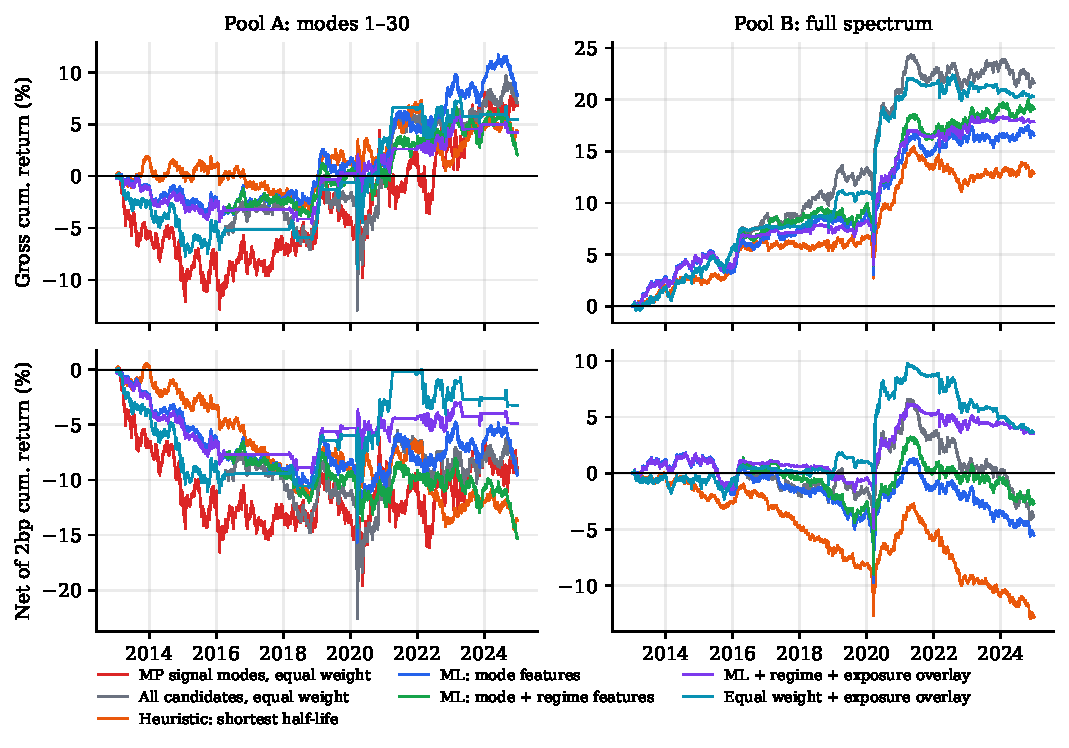
\includegraphics[width=\textwidth]{cumulative_pnl}
\caption{Cumulative log returns per unit gross exposure, before (top) and
after (bottom) 2~bp costs.}
\label{fig:pnl}
\end{figure}

\paragraph{The original specification fails.} The original repository
strategy (daily-return reversal on the top 20 signal modes, raw-return
projection) has a gross Sharpe of \GSROrig{}. With daily turnover of
\TOOrig{} times its book it loses heavily after costs (net Sharpe
\SROrig). Its failure is predicted by \cref{tab:spectrum}: it trades the
part of the spectrum that does not revert, with a signal that is
negative there.

\paragraph{Gross reversion is real, but small relative to turnover.}
Trading every Pool~B mode with equal risk earns a gross Sharpe of
\GSREWB{}, and does so with almost no market exposure. Per unit of gross
exposure, however, the return is only \GRetEWB\% a year against daily
turnover of \TOEWB, a break-even cost of \BEEWB~bp. At 2~bp the net
Sharpe is \SREWB. Pool~A is weaker throughout (gross \GSREWA). The
long-short book is extremely diversified, so its volatility per unit
gross is low (\VolEWB\%), and a levered implementation would scale return
and volatility together. Costs, not risk, are the binding constraint.

\paragraph{ML selection beats random selection, not diversification.}
In Pool~B, the ML-selected top third has a gross Sharpe of
\GSRMLAllB{}. A randomly selected top third of the same size averages
\PlaceboMeanB{} net (95th percentile \PlaceboNFB), and the ML strategy
beats every one of 200 random draws ($p<0.005$). But the ML strategy
does not beat simply trading all candidates. The Sharpe difference
against equal weight is \DiffMLAllB{} (bootstrap $p=\DiffPMLAllB$), and in
Pool~A it is negative (\DiffMLAllA). Holding all modes diversifies
away more noise than a weak classifier can add by choosing among them.
The half-life heuristic is significantly \emph{worse} than equal weight
in Pool~B (\DiffHeurB, $p$ for improvement $=\DiffPHeurB$).

\paragraph{Regimes matter most.} Reversion makes money in the stress
state and loses in the calm state, for every strategy and both pools.
For the Pool~B equal-weight portfolio the Sharpe ratio is
\RegSREWBStress{} in stress and \RegSREWBCalm{} in calm. This matches
the evidence that short-term reversal profits are a compensation for
liquidity provision that rises with volatility
\citep{nagel2012,khandani2011}. The overlay, which learns this
asymmetry walk-forward, raises the net Sharpe of the equal-weight Pool~B
portfolio to \SREWOverB{} (difference \DiffEWOverB, $p=\DiffPEWOverB$).
Combined with ML selection it reaches \SRMLOverB{} (\DiffMLOverB,
$p=\DiffPMLOverB$) and reduces the maximum drawdown from \DDEWB\% to
\DDMLOverB\%. Part of the gain comes from lower turnover, since the
overlay often trades at reduced size. The gross Sharpe also rises, to
\GSRMLOverB.

\subsection{Robustness}
\label{sec:robustness}

\begin{figure}[t]
\centering
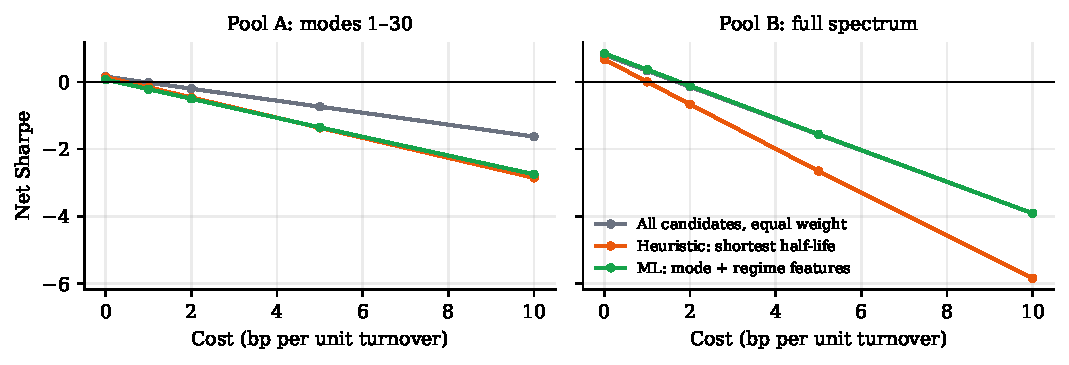
\includegraphics[width=\textwidth]{costs}
\caption{Net Sharpe ratio as a function of the cost per unit turnover.}
\label{fig:costs}
\end{figure}

\begin{table}[t]
\centering\small
\caption{Robustness of the primary ML strategy (logistic, mode + regime
features, top third, no overlay) and the equal-weight benchmark. Net
Sharpe at 2~bp, with gross Sharpe in parentheses. Rows below the rule
re-build the episodes and re-train the models; sub-period rows split
the baseline run.}
\label{tab:robustness}
\resizebox{\textwidth}{!}{\begin{tabular}{lrrrrrr}
\toprule
 & \multicolumn{3}{c}{Pool A: modes 1--30} & \multicolumn{3}{c}{Pool B: full spectrum} \\
\cmidrule(lr){2-4}\cmidrule(lr){5-7}
Test & ML & EW & AUC & ML & EW & AUC \\
\midrule
Baseline ($W$=252, $L$=60, $H$=21) & -0.50 (0.07) & -0.20 (0.16) & 0.521 & -0.12 (0.85) & -0.14 (0.81) & 0.514 \\
\midrule
Sub-period 2013--2016 & -1.27 (-0.42) & -0.92 (-0.37) & -- & 0.04 (1.48) & 0.04 (1.61) & -- \\
Sub-period 2017--2019 & -0.20 (0.51) & -0.29 (0.23) & -- & -0.74 (0.66) & -0.34 (1.05) & -- \\
Sub-period 2020--2021 & -0.05 (0.34) & 0.30 (0.52) & -- & 0.44 (1.03) & 0.56 (1.09) & -- \\
Sub-period 2022--2024 & -0.65 (-0.11) & -0.19 (0.19) & -- & -0.49 (0.47) & -1.20 (-0.12) & -- \\
Select top 20\% & -0.63 (-0.04) & -0.20 (0.16) & -- & -0.25 (0.82) & -0.14 (0.81) & -- \\
Select top 50\% & -0.42 (0.07) & -0.20 (0.16) & -- & -0.08 (0.85) & -0.14 (0.81) & -- \\
Model: GBM & -0.65 (-0.16) & -0.20 (0.16) & -- & -0.56 (0.41) & -0.14 (0.81) & -- \\
Model: RF & -0.36 (0.15) & -0.20 (0.16) & -- & -0.54 (0.64) & -0.14 (0.81) & -- \\
Execution delay +1 day & -0.53 (0.01) & -0.27 (0.10) & 0.514 & -0.74 (0.33) & -0.59 (0.42) & 0.508 \\
Window $W=126$ & -0.60 (-0.01) & -0.24 (0.15) & 0.521 & -0.63 (0.35) & -0.28 (0.36) & 0.516 \\
Window $W=504$ & -0.58 (-0.10) & -0.10 (0.24) & 0.510 & -0.13 (0.87) & -0.31 (0.83) & 0.519 \\
Lookback $L=20$ & -0.70 (0.19) & -0.43 (0.24) & 0.507 & -0.97 (0.64) & -0.36 (0.97) & 0.513 \\
Lookback $L=120$ & -0.66 (-0.13) & -0.21 (0.03) & 0.519 & -0.82 (0.55) & -0.13 (0.60) & 0.521 \\
Holding $H=10$ & -0.31 (0.45) & -0.07 (0.30) & 0.524 & -1.22 (0.64) & -0.44 (0.72) & 0.518 \\
Holding $H=42$ & -0.35 (0.17) & -0.26 (0.09) & 0.510 & -0.24 (0.63) & -0.12 (0.66) & 0.517 \\
\bottomrule
\end{tabular}}
\end{table}

\Cref{fig:costs,tab:robustness} summarize the sensitivity analysis.
Net results are fragile to costs: at 5~bp every strategy has a clearly
negative Sharpe (Pool~B equal weight: \SRCostFiveEWB), and at zero cost
the Pool~B equal-weight Sharpe is \SRCostZeroEWB. Adding one day of
execution delay roughly halves the gross Sharpe ratio in Pool~B (from
\GSREWB{} to 0.42 for equal weight, and from \GSRMLAllB{} to 0.33 for
ML; \cref{tab:robustness}). A large share of the measured reversion is
therefore a one-day effect, consistent with close-to-close bid--ask bounce and
short-lived liquidity shocks. Strategies that cannot trade at the
close would capture much less of it. In Pool~B the gross Sharpe ratio stays positive in every
re-specification (window, lookback, holding period, selection fraction,
model), but the ML strategy beats equal weight net of costs only in a
few of them (e.g.\ $W=504$ or selecting the top half). In Pool~A gross
Sharpe ratios are near zero throughout. Gross performance is strongest
in 2013--2016 and 2020--2021 and weak in 2022--2024. Gradient boosting
and random forests produce worse strategies than the logistic model,
despite similar AUCs.
